% Copyright (c) 2014,2016 Casper Ti. Vector
% Public domain.

\chapter{研究動機}
%\pkuthssffaq % 中文测试文字。
	\section{密碼貨幣的發展}
	追溯著加密貨幣市場的演進,於2009年時,比特幣並非第一個密碼貨幣,在比特幣之前已經有著很多的類似的密碼貨幣開發實驗,但是一直無法做出一個穩定點對點式的電子現金系統,至於製作貧頸會在後段章節中闡述。在比特幣穩定發展之後,有著許多對比特幣有興趣的研究者,以穩定的比特幣系統為基礎修改了許多基本的協議。於2011年相繼創造出了貨幣就稱之為山寨幣,山寨幣早期較為著名的有萊特幣(LiteCoin,LTC)\parencite{litecoin}、狗幣(DogeCoin,DOGE)\parencite{dogecoin}、域名幣(NameCoin,NMC)\parencite{namecoin},於2014年也有人認為比特幣挖礦使用到了大量的哈希運算,這樣的大量運算也浪費了許多的社費資源,努力的開發具有意義的工作量證明挖礦算法較為著名的有素數幣(Primecoin,XPM)\parencite{primecoin}。 於2015年底也誕生了現在最為著名的以太坊經典(Ethereum Classic,ETC)\parencite{ethereumclassic}、以太坊(Ethereum,ETH)\parencite{ethereum},使得區塊鏈技術不再僅僅只是一個點對點的電子現金系統,以太坊最重大突破設計在於將編程語言虛擬機,移植到了區塊鏈架構上,也創造出了屬於乙太坊的編程語言Solidity,使得再以太坊的虛擬機當中,可以用Solidity創建智能合約,合約可以建構去中心化的應用程序,如去中心化的交易所。

	\section{密碼貨幣市場(Cryptocurrency Market)}
	密碼貨幣最具代表性的是比特幣,但除了比特幣之外也有著許多模仿比特幣的密碼貨幣,有的是為了利益,有的是鑒於比特幣的各種不完美,希望可以解決比特幣不足之處。密碼貨幣市場中有成千上萬種的密碼貨幣,較為著名的密碼貨幣會在Cryptocurrency Market Capitalizations\parencite{CryptocurrencyMarketCapitalizations}的排行榜中出現,截至2018年2月8日該排行榜已經收入了1510種密碼貨幣。在Cryptocurrency Market Capitalizations統計的數據當中,可知整體的密碼貨幣市場,如下圖\ref{TotalMarketCapitalization}所示,於2018年1月7日創下了歷史新高,密碼貨幣市場的總市值也高達了829,579,000,000美金,相當於五兆人民幣的總市值。

		\begin{figure}[h]
			\centering
			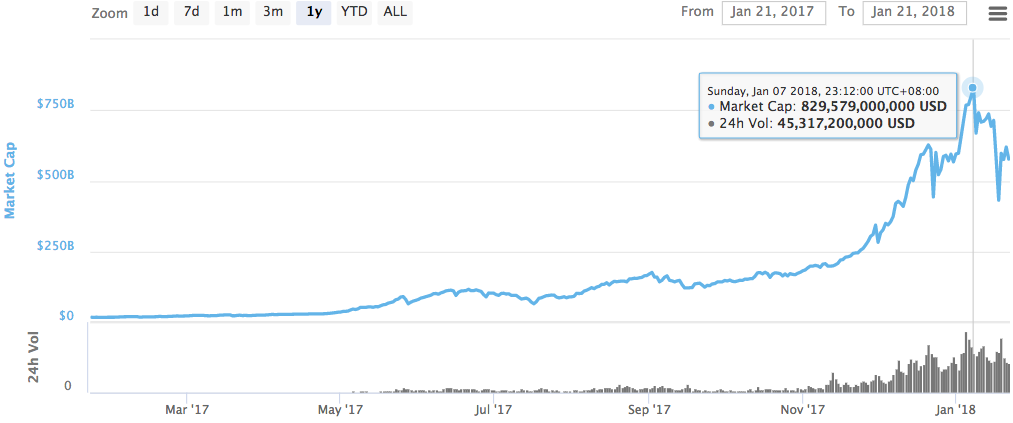
\includegraphics[width = .9\textwidth]{TotalMarketCapitalization.png}
			\caption{Total Market Capitalization\parencite{CryptocurrencyMarketCapitalizations}}\label{TotalMarketCapitalization}
		\end{figure}

	經由Cryptocurrency Market Capitalizations數據顯示,自2013年起已經高達150億美金,2014年與2015年間總市值減少到近乎2013年的一半,於"Have the security flaws surrounding BITCOIN effected the currency's value?."
	論文\parencite{HavethesecurityflawssurroundingBITCOINeffectedthecurrencysvalue?}
	中做了詳盡的比特幣市場調研,致力於探討在各個比特幣市場大事件中對比特幣價格的波動影響,針對影響的程度該論文給出影響指數,當中影響最為嚴重的是於2014年2月發生的日本交易所Mt.Gox倒閉事件,因為早期的密碼貨幣市場中無完善的法律規範,各國對密碼貨幣的接受度有所不同,日本對金融科技的接受度相較較為開放的情況下成立了全世界第一家比特幣交易所,也因為交易所不夠普及,使得大部分的密碼貨幣交易都集中在Mt.Gox交易所中,促使Mt.Gox倒閉事件會成為影響市場價格重大因子之一,也造成2014與2015年的密碼貨幣市場的低迷,2017為2016年的35倍成長幅度,主要是因為美國最大的期權交易中心芝加哥期權交易所於	2017年12月10日支持比特幣期貨,將比特幣價格推升到20,000美金的歷史新高,下圖\ref{Thetotalmarketcapitalization}為2013年至2018年歷年的密碼貨幣總市值的統計圖表。

		\begin{figure}[h]
			\centering
			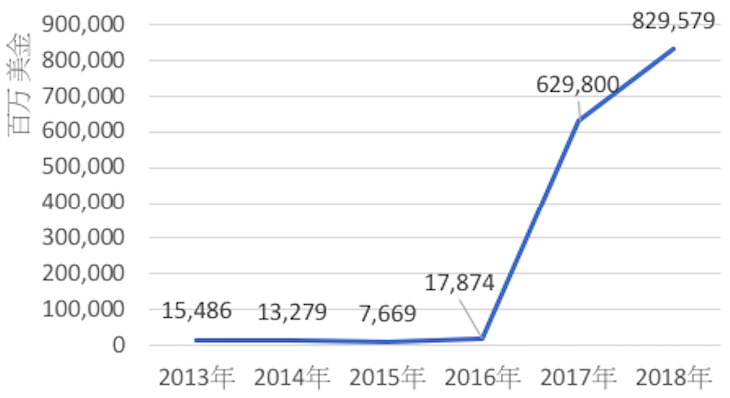
\includegraphics[width = .7\textwidth]{Thetotalmarketcapitalization.png}
			\caption{密码货币历年最高总市值\parencite{CryptocurrencyMarketCapitalizations}}\label{Thetotalmarketcapitalization}
		\end{figure}
	

	\section{密碼貨幣的優勢}
	於2009年Satoshi Nakamoto發布了比特幣系統,成為全世界第一個密碼貨幣的雛形。密碼貨幣的特點在於24小時不間斷運作、遠距離支付、貨幣為使用者持有

		\subsection{24小時不間斷運作}
		基於區塊鏈技術與點對點網路的架構,以比特幣為例,自2009年至今,所有的比特幣交易事件皆會儲存在比特幣區塊鏈當中,區塊鏈既無法刪除也無法修改,比特幣區塊鏈會以點對點網路的方式儲存在比特幣網路中的全節點,目前比特幣網路中的全節點高達10552個。與傳統中心化的銀行數據庫相比,可能會因為銀行的服務器維護,導致交易無法順利進行,甚至可能有黑客的入侵導致銀行或是個人資產有重大的損失。點對點網路提供穩定的數據庫資料元,不會因為數據庫的關機而無法繼續使用,
		
		\subsection{遠距離支付}
		於跨國匯款從美國轉帳至中國一百萬美金的場景中,需要經過的手續較為繁瑣,資金有可能需要經過多個國家才可以抵達目的地,在經過各個國家的過程中,需要支付各國的手續費,也需要等待各個國家辦理該業務的時間,既使當資金順利抵達了目的地的銀行,目的地的銀行也需要花將近三至五日的工作日確認該筆金額的來源。屆時領款人亦需要前往銀行完整的身份驗證、解釋資金用途,才得以取得這筆的跨國資金。比特幣系統當中,有著24小時不間斷運作的優點,也因為點對點網路架構,使得比特幣無需經由傳統的金融機構繁瑣的步驟完成國際匯款,於比特幣系統中無系統壅塞的清況下,平均10分鐘即可入帳。

		\subsection{貨幣為使用者持有}
		傳統的金融體系中,資金的存儲、流動往往需要經過銀行,百姓將所有的資產存入銀行,拿到的是一串數字的銀行餘額,銀行是一個中心化的機構,有著最高的權利。中央社的新聞\parencite{Bankguardsstolen}指出,台灣各地於2017年接連於土地銀行、日盛銀行、彰化銀行、京城銀行、兆豐銀行皆傳出銀行行員監守自盜的行為,總金額高達一億三千為新台幣。在比特幣系統中,比特幣有如金幣般存放在個人的比特幣地址當中,使用者為真實持有著貨幣,既使是比特幣系統皆無法動用該筆比特幣資產,唯有比特幣地址的私鑰持有者,才可以移動該筆資產。

	\section{密碼貨幣的劣勢}
% vim:ts=4:sw=4
